\section{PolyHashing: Integrity Verification}
\label{sec-polyhashing}

\begin{figure}
\center
% We need pdflatex with png images. Plain latex would fail here.
% So, we conditionally include this so we can still build with latex,
% just without this image.
%\begin{minipage}[b]{\linewidth}
\hspace{-4mm}
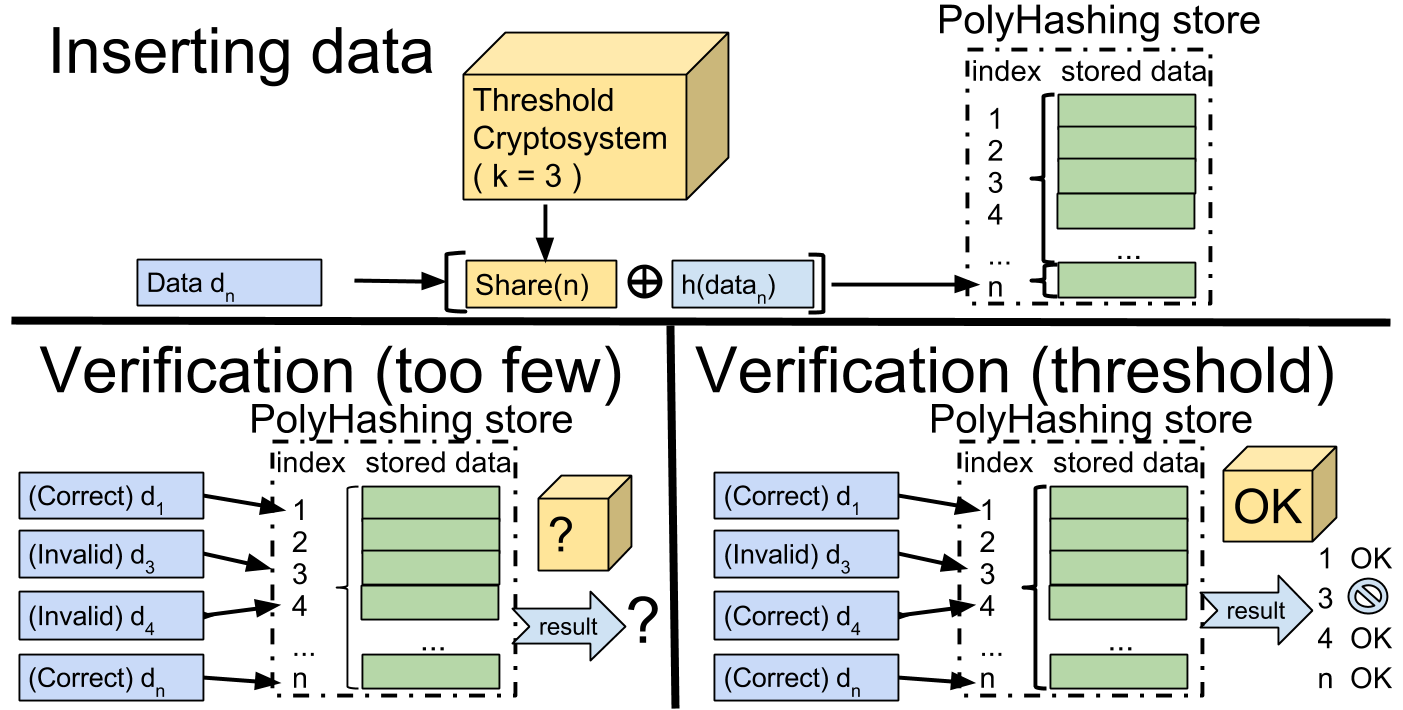
\includegraphics[width=1.05\columnwidth]{figures/polyhashing.png}
%\end{minipage}
\caption{This figure demonstrates inserting data and integrity verification 
for PolyHashing.   In the case of data verification, the caller performs 
PolyHashing verification on values simultaneously.  Only if at least the 
threshold of correct values are provided (3), can 
the threshold cryptosystem be decoded and any value be checked. Note that the
caller does not know whether data values are correct or invalid when calling
the verification routine.   Only the data in the dashed box is persisted
on disk.}
\label{fig-polyhashing}
\end{figure}


%Traditionally, a threshold cryptosystem is used to hide 
%information so that multiple parties must come together to recover the 
%original data.  With PolyHashing, there is a single party with all data, but
%the threshold system obscures hash information so that values may only be 
%checked if a threshold of correct values are known.
%To achieve these properties, PolyHashing combines two techniques: a threshold
%cryptosystem and a hash function.   


PolyHashing is a general technique for concurrently verifying the integrity of 
a set of values.% (the next section discusses how to apply PolyHashing to the
%specific problem of protecting passwords).   
The purpose of PolyHashing is 
much like using a traditional hashing function and storing 
the hash of a value $h(v_i)$ in the store at a specific index $i$.   However, 
with PolyHashing, the hash values are blinded so that
integrity verification may only be performed if a threshold $k$ of the values 
are provided.   If less than the threshold of correct $h(v)$ items 
are provided, {\bf no information about which values are correct is leaked.}   


These properties are provided by leveraging a threshold cryptosystem 
(Figure~\ref{fig-polyhashing}).   Each entry in a PolyHashing store is XORed 
with a share.   If a threshold of correct values are provided, then the 
attacker can recover enough shares to recover the secret.   By using
interpolation, all shares to be computed and thus any hash can be 
validated.  As such, a PolyHashing store has information-theoretic 
confidentiality when 
less than the threshold of values are known, but can validate the 
integrity of values individually if at least $k$ of them are known.


When a blank PolyHashing store is created, the threshold $k$ is given.  
A cryptographically random value is used to seed all shares in the
threshold cryptosystem.  For example, when using Shamir Secret Sharing for 
PolyHashing, the constant term (which is typically the stored secret) is 
randomly generated.   In this case, the purpose of the threshold cryptosystem 
is not to store a secret, but instead to act like a one-time pad to obscure 
the hashes that are stored.   As such the length of shares generated by 
the threshold cryptosystem should be equal to the length of the hashes.


To add a secret to the store (the top of Figure~\ref{fig-polyhashing}), one 
will compute an index $i$ (to 
later locate which secret in the store corresponds to this entry) and
the hash of the data.   The value $i$ is also used as the 
share number in the Shamir Secret Store for computing the $f(x)$ values of the
shares.   To store an item, the party will add an entry that includes the 
identifier, share number, and the XOR of the $f(x)$ values 
with the hash.   %If desired, a single secret can have more
%than one share by choosing a unique  and share number and repeating
%the process.   



If a party possesses the PolyHashing store, they cannot validate any hash 
value without at least $k$ correct hash values (the bottom left of 
Figure~\ref{fig-polyhashing}) because they do not have enough hashes
to recover the threshold
cryptosystem's shares.  When a party has $k$ or more hash 
values (bottom right of Figure~\ref{fig-polyhashing}), they can 
uncover all shares of the threshold cryptosystem and validate all hash
values.   As a result, other requests can be validated by computing
the hash of the value $h(v_i)$, XORing the $i$th share, and
comparing the result with the stored data in the PolyHashing store.

Note that the threshold cryptosystem's shares are not stored on disk or 
otherwise transmitted.   Once enough correct values are known by a party, by 
XORing the $h(v)$ values with the data in the PolyHashing store, one can 
recover a threshold of shares.   This allows the party to reconstruct all
data in the threshold cryptosystem's store.   By keeping this information
only in memory on a running system, an attacker that can read the disk 
contents but does not know a threshold of correct values cannot validate
the correctness of values individually.

More formally, given an information-theoretic $(k,n)$-threshold cryptosystem 
with shares $S=\{s_0, ... s_n\}$ that stores values $H=\{h(d_0), ... h(d_n)\}$.
Suppose that $length(s_i) = length(h(x))$. A PolyHashing 
store $Z$ has items $Z=\{z_0, ...z_n\}$ such that $z_i= s_i \oplus h(d_i)$.   

{\bf Theorem:} $Z$ provides information-theoretic 
privacy for unknown items in $H$ when $k-1$ items from $H$ are known.


{\bf Proof:}
Suppose that $h(d_j)$ is an item that is not in the set of $k-1$ known items.
Since $S$ is a $(k,n)$-threshold cryptosystem and the observer knows only 
$k-1$ items, they only know $k-1$ shares of $S$.   Thus they cannot recover 
$S$ from the known shares of $S$.   Therefore $s_j$ has information-theoretic 
privacy.   Since $z_j$ is 
the result of XORing $s_j$ with another value of the same length, $s_j$ acts 
like a one-time pad for $h(d_j)$.   Thus, $z_j$ reveals no information
about $h(d_j)$.   However, since the choice of $j$ was 
arbitrary, the same argument applies to all of the $n-(k-1)$ unknown items in 
$H$ and clearly no information about $h(d_j)$ is revealed by any $z_i$ where
$i \neq j$.  
$\blacksquare$



